% file: modeledsystems.tex

\chapter{Modeled systems}
The goal of this thesis is to study fracture of methane hydrates. In order to do that, I need to know the mechanical properties of the model I study. Since studies of mechanical properties of methane hydrates modeled with TIP4P/ICE+UAM are scarce, I start this chapter by working out even the basic properties of the model, such as Poissons ratio and Youngs modulus. In order to be sure that the methods I use to estimate the mechanical properties work, I first check them with known values for a Lennard-Jones crystal. 

\section{Shear viscosity and diffusivity of the water model}
I have not been successful in finding values for the shear viscosity and diffusivity of bulk liquid water modeled with TIP4P/ICE. To measure these properties, I run a simulation like the one I ran to calculate verify the same properties for the TIP4P/2005 potential. Figure \ref{fig:viscosity_green_kubo_tip4p_ice} shows the Green-Kubo relation for the viscosity using 5 independent pressure components from 4 indepentent simulations with different simulation box sizes. Based on these data, I estimate the shear viscosity of TIP4P/ICE to $\eta_{GK} = \text{\SI{1.63\pm 0.05}{\milli\pascal\second}}$. 

\begin{figure}
\centering
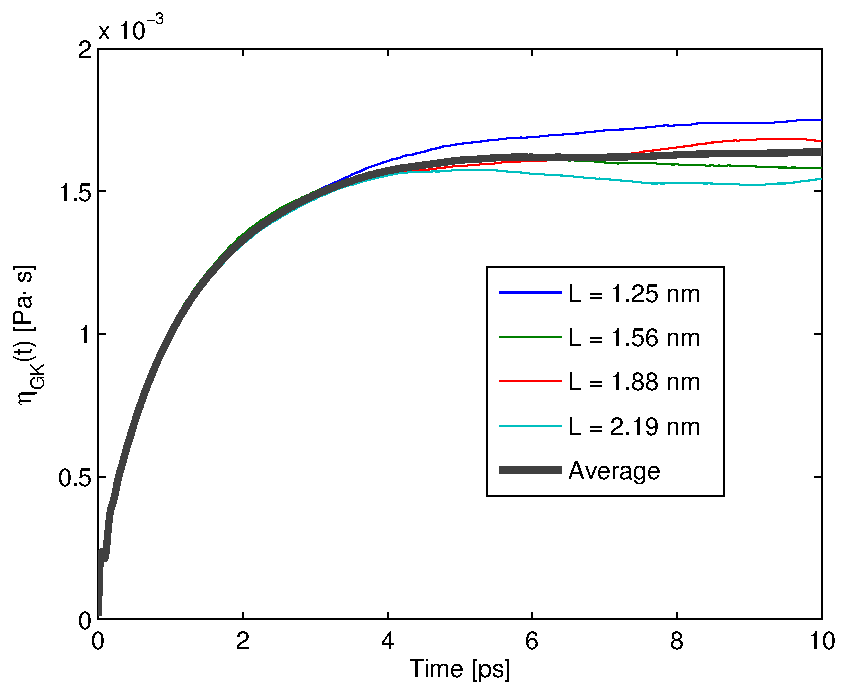
\includegraphics[width=10cm]{../figures/thesis/viscosity_green_kubo_tip4p_ice.pdf}
\caption{Shear viscosity for TIP4P/ICE at \SI{300}{\kelvin} and $\rho = \text{\SI{0.98}{\gram\per\cubic\cm}}$. Each thin line shows the average of the 5 independent pressure component. The thich line is the average of 4 independent simulations. The viscosity is estimated to $\eta_{GK} = \text{\SI{1.63\pm0.05}{\milli\pascal\second}}$}
\label{fig:viscosity_green_kubo_tip4p_ice}
\end{figure}

\begin{figure}
\centering
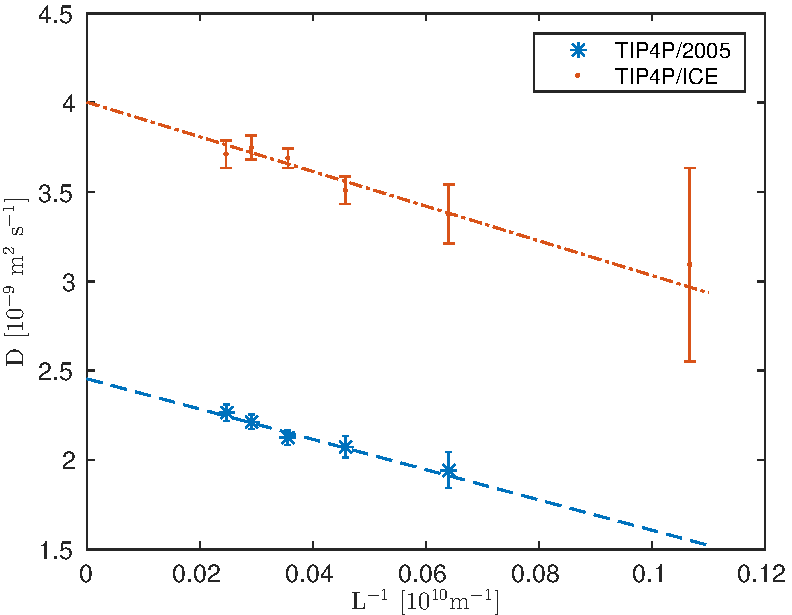
\includegraphics[width=10cm]{../figures/thesis/diffusivity_comparison_tip4p_ice_2005.pdf}
\caption{Linear regression of self diffusion coefficients as a function of inverse simulation box length. Results for TIP4P/2005 (blue) were already reported in the verification section. The self-diffusion coefficient for TIP4P/ICE is estimated to $D_0 = \SI{4.0 \pm 0.1 d-9}{\meter\squared\per\second}$}
\label{fig:diffusivity_comparison_tip4p_ice_2005}
\end{figure}

\section{Measuring elastic properties with a constant strain rate}
A naive approach, which i will use for crude estimates, is to subject a system to a constant strain rate by expanding the simulation box in one of the coordinate directions, and rescale all atom positions accordingly. An anisotropic thermo-barostat should be applied along the other axes, to keep the environment pressure and temperature constant. Since the barostat scales the simulation box, strains along the two axes perpendicular to the applied strain can be measured as the contraction of the simulation box in these directions:

\begin{equation}
\varepsilon_i = \frac{L_i-L_{0, i}}{L_{0, i}}
\end{equation}

If the sample is isotropic, I only have to simulate strain application in one of the coordinate directions to estimate both Young's modulus and Poissons ratio for a given system. To account for the possibility that the model I use do not exhibit isotropic behavior, I will check strains in both of the coordinate axes that are perpendicular to the axis of applied strain when calculating Poissons ratio. The scalar value of $\nu$ is the slope of the strain-strain curve, and for $E$ of the stress-strain curve, both in their linear regions. I will calculate these slopes using linear regression with least squares on the curves.
In the following, I will apply the method described above to a Lennard-Jones crystal and to the TIP4P/ICE+UAM methane hydrate model.

\subsection{Lennard-Jones crystal}
The FCC-lattice with a Lennard-Jones potential has been extensively investigated due to its simplicity. Therefore it provides robust benchmarking capabilities. I want to check that my protocols for dynamic (but quasistatic) determination of elastic properties and fracture strength reproduces known parameters for a Lennard-Jones solid. Reference values are for Young's modulus, $E=61.1 \epsilon/\sigma^3 = \text{\SI{2.40}{\giga\pascal}}$ (for the parameters I use for Methane), and for Poissons ratio, $\nu=0.347$. Values are taken from a molecular dynamics study by Quesnel et al. \cite{Quesnel1993}.

Figures \ref{fig:stress_strain_11_11_11_and_22_22_22_y_z_poisson_lennard_jones} and \ref{fig:strain_strain_11_11_11_and_22_22_22_y_z_poisson_lennard_jones} show data for a strain test of two systems of Lennard-Jones particles subjected to a strain rate of \SI{2d-8}{\per\femto\second} over \SI{0.8}{\nano\second} resulting in a maximum strain of \SI{0.8}{\percent}. The external pressure was set to \SI{50}{\mega\pascal}, and the temperature was \SI{5}{\kelvin}. Along with the data are estimates of Poissons ratio and Young's modulus, taken as the best linear regression with least squares. 


\begin{figure}
\centering
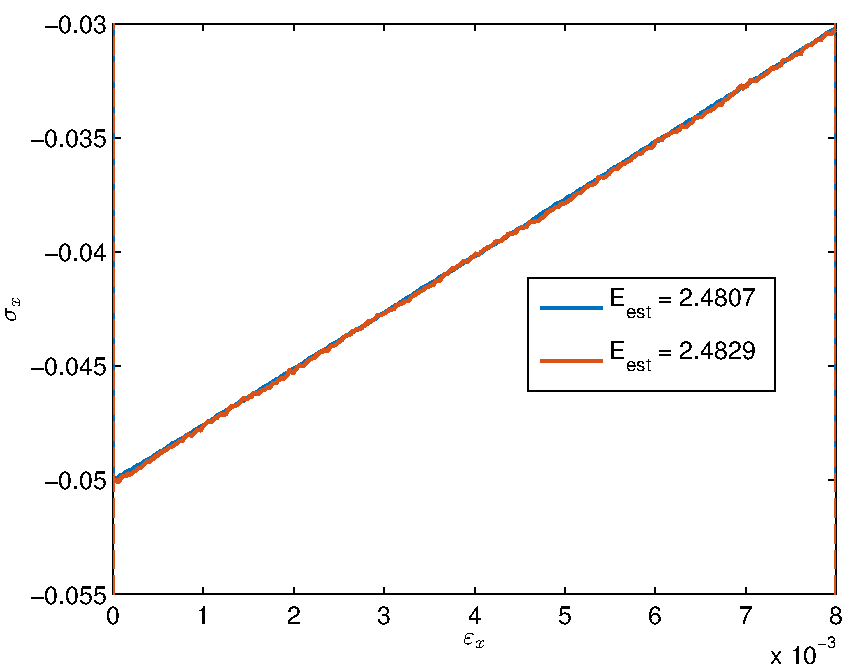
\includegraphics[width=10cm]{../figures/thesis/stress_strain_11_11_11_and_22_22_22_y_z_poisson_lennard_jones.pdf}
\caption{Stress-strain relations for Lennard-Jones systems of $11^3$ (red) and $22^3$ (blue) FCC unit cells. The sample was subjected to a constant strain rate of \SI{2d-8}{\per\femto\second}. $E$ is estimated using linear regression with least squares on all data points.}
\label{fig:stress_strain_11_11_11_and_22_22_22_y_z_poisson_lennard_jones}
% Path to simulation: /media/henriasv/Data/molecular-data/master_methane_hydrates/stress_strain/20150113_lennard_jones_strain
\end{figure}

\begin{figure}
\centering
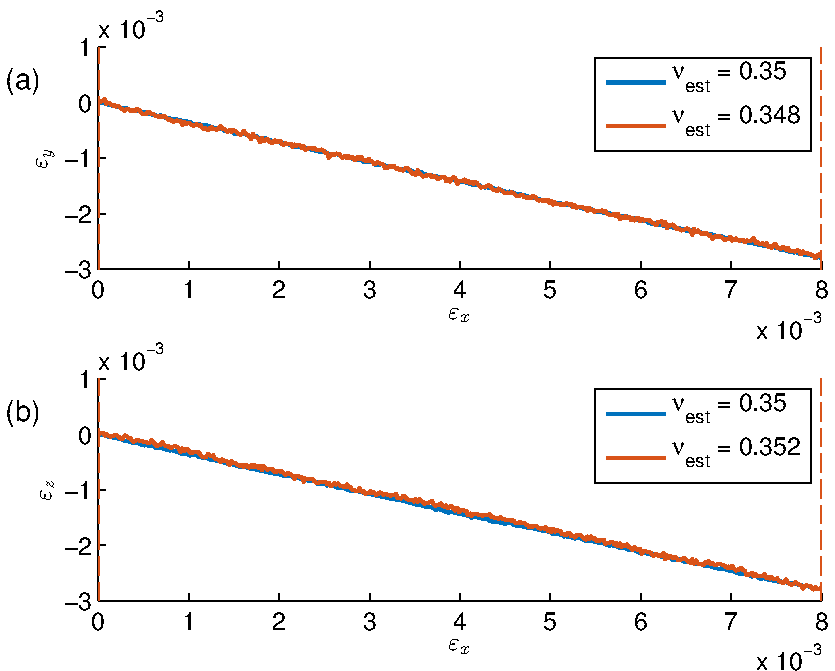
\includegraphics[width=10cm]{../figures/thesis/strain_strain_11_11_11_and_22_22_22_y_z_poisson_lennard_jones.pdf}
\caption{Strain-strain relations for for the same simulations as in Figure \ref{fig:stress_strain_11_11_11_and_22_22_22_y_z_poisson_lennard_jones}. All data points were used to estimate $\nu$.}
\label{fig:strain_strain_11_11_11_and_22_22_22_y_z_poisson_lennard_jones}
% Path to simulation: /media/henriasv/Data/molecular-data/master_methane_hydrates/stress_strain/20150113_lennard_jones_strain
\end{figure}

\subsection{S1 methane hydrate with TIP4P/ICE+UAM}
To my knowledge, there are no published estimates of Youngs modulus and Poissons ratio for the TIP4P/ICE+UAM model of methane hydrates. Therefore, I seek to make crude estimates of these quantities in dynamic simulations. I apply a constant strain rate by continously rescaling particle positions in one direction during MD-simulations. The other directions are kept under a constant pressure with anisotropic barostatting.
Figure \ref{fig:stress_strain_11_11_11_tip4p_ice_uam} shows the stress strain relationships and corresponding estimates of Youngs modulus for a system of 11x11x11 S1 unit cells subjected to strain rates of \SI{5d-7}{\per\femto\second} and \SI{2d-7}{\per\femto\second}. By extrapolating the results to quasistatic strain, Youngs modulus is estimated to \SI{7.1}{\giga\pascal}. 
Figure \ref{fig:strain_strain_11_11_11_y_z_poisson_tip4p_ice_uam} shows the relationship between applied strain along the x-axis and the measured strain along the other axes. It is not outrageous to assume S1 methane hydrate to be isotropic. Under this assumption, and by extrapolation to quasisatic strain, I estimate the poisson ratio for this model of S1 methane hydrate to be $\nu = 0.41$. 

\begin{figure}
\centering
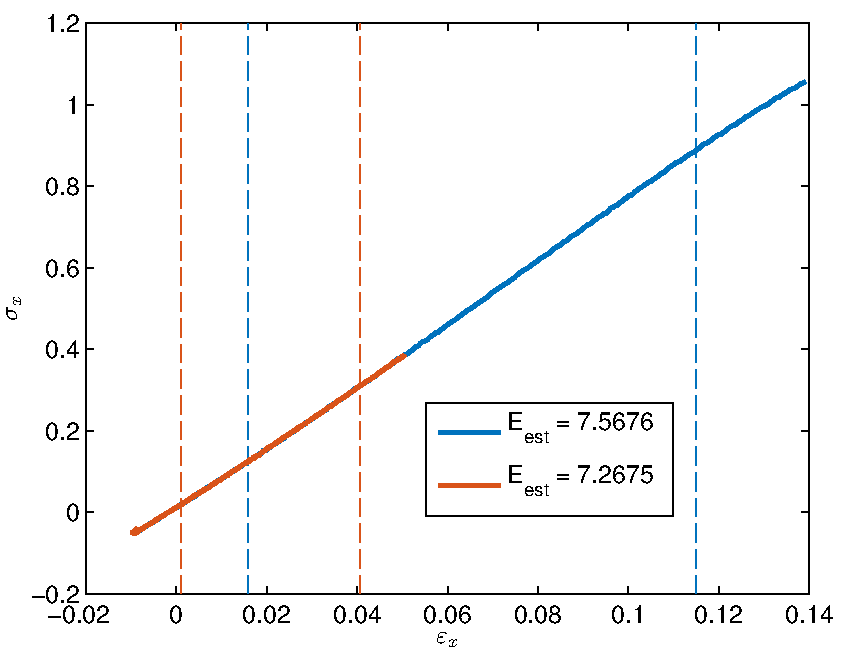
\includegraphics[width=10cm]{../figures/thesis/stress_strain_11_11_11_tip4p_ice_uam.pdf}
\caption{Stess-strain relations for a system of 11x11x11 S1 unit cells. Dashed lines indicate the region that was used to estimate Youngs modulus. Strain rates of \SI{5d-7}{\per\femto\second} (blue) and \SI{2d-7}{\per\femto\second} (red) along the x-axis. Upon close visual inspection, a slight rising slope can be seen for small strains and a rising slope for large strains, but overall the stress-strain relation is suprisingly linear, especially given the large strain-range.}
\label{fig:stress_strain_11_11_11_tip4p_ice_uam}
% Path to simulation: /media/henriasv/Data/molecular-data/master_methane_hydrates/stress_strain/20150108_youngs_modulus

\end{figure}

\begin{figure}
\centering
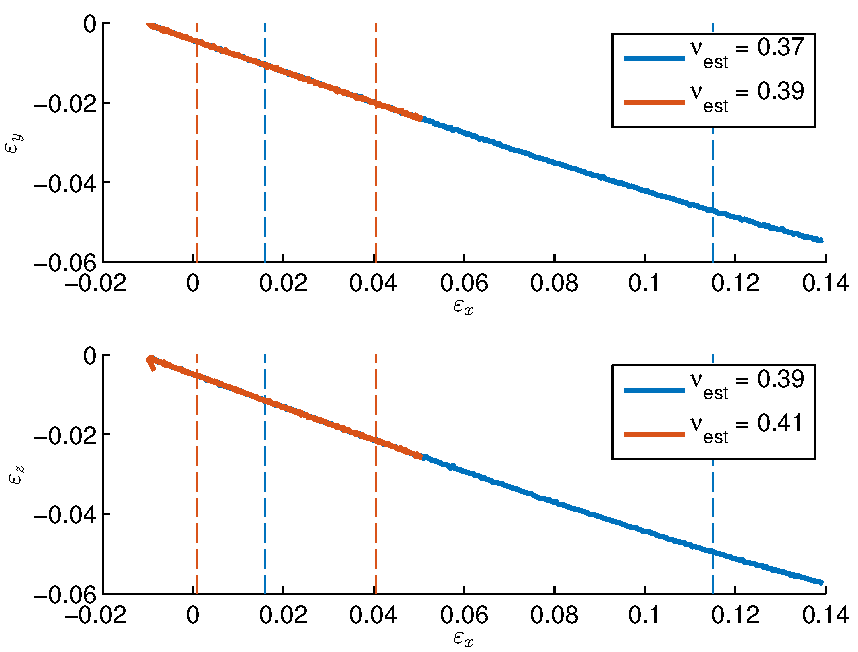
\includegraphics[width=10cm]{../figures/thesis/strain_strain_11_11_11_y_z_poisson_tip4p_ice_uam.pdf}
\caption{Strain-strain relations for the same system as in Figure \ref{fig:stress_strain_11_11_11_tip4p_ice_uam}. Measured strain along the y-axis (a) and z-axis (b) is plotted against the applied strain along the x-axis. Dashed lines indicate the region that was used to estimate Poissons ratio.}
\label{fig:strain_strain_11_11_11_y_z_poisson_tip4p_ice_uam}
% Path to simulation: /media/henriasv/Data/molecular-data/master_methane_hydrates/stress_strain/20150108_youngs_modulus

\end{figure}

\section{Fracture and fracture toughness}

\subsection{Determining the critical stress intensity factor}
As described in the section about fracture mechanics, the stress intensity factor is commonly used to calculate the fracture toughness of a material. The critical energy release rate is usually defined as:
\begin{equation}
	G_C = -\left(\frac{\partial P}{\partial A_{\text{crack}}}\right)_{T, \text{loading}}
	\label{eq:def_critical_energy_release_rate}
\end{equation}

I will follow the method of \cite{Hantal2014} to calculate the critical stress intensity factor (This method was used for illite with ClayFF and ReaxFF):\begin{equation}
	G_C = V \frac{\int_0^{E_{\text{final}}}\uuline{\Sigma}(E) : \dd \uuline{E}}{\int_0^{E_{\text{final}}} \dd A_{crack}}
	\label{eq:hantal_critical_energy_release_rate}
\end{equation}

This is in principle sufficient to determine the critical energy release rate for any mode of loading, provided that the conditions for using Equation \ref{eq:hantal_critical_energy_release_rate} to estimate the critical energy release rate are met.

\subsection{Simulation details}
@VerifyThatThisIsADescriptionOfHantal2014
It is not at all obvious how to perform simulations to determine the fracture toughness. \citet{Hantal2014} performed NVT simulations and imposed a series of small deformations to their sample. After each deformation, they minimized the system, and then ran molecular dynamics for \SI{10}{\pico\second}. I have tried to use the same protocol, but find that for my system, the impact on the energy distribution among the degrees of freedom is too large when performing minimizations between the deformations. this results in a system farther out of equlilibrium that the deformed but not minimized system. Therefore, a possible protocol:

\begin{enumerate}
\item Equilibrate the system NVT (Molecular dynamics)
\item Perform small deformation
\item Reequilibrate the system NVT (Molecular dynamics)
\item If the strain i low: Return to 2. If the strain is high: continue.
\item Molecular dynamics run to wait for failure
\item If failure does not occur, or crack length stabilizes: Return to 2. 
\end{enumerate}

However there are problems here: The waiting time when waiting for failure must be carefully chosen, and if it turns out that critical and sub-critical failure are hard to distinguish, or even impossible to define, then waiting times can be arbitrarly long. 

From the latter discussion, I propose to exploit the possible time problem, and investigate the dependence on strain and temperature on the crack velocity and the waiting time before fracture occurs. The latter is possibly computationally expensive to get sufficient statistic to make any confident statements. 

A simpler protocol -- and I believe this to be a good way to study this particular system -- is to subject the sample to a constant strain rate, then wait for a crack to propagate. This is simple to do, and is also close to experimental conditions. The downside is that the loading is varying during fracture, disturbing measurements of properties like crack velocity at constant loading. It is, however, reasonable to believe that at low strain rates, these effects will be small, if not negligible. This can also be solved by setting the strain rate to zero at some predefined strain level, which is estimated from experience, and can be systematically varied. 


\subsection{Proof-of-concept simulations}
Before performing serious simulations, I do preliminary simulations to find out whether the protocol proposed in the latter section can produce interesting results. I do simulations on a relatively small and quasi 2-dimensional system -- the system is only one unit cell thick -- to keep computational costs down. The total computational cost for tuning in on parameters and getting rid of bugs and blunders was about $10^4$ cpu hours.

Figure \ref{fig:proof_of_concept_crack} shows the potential energy and strain for four simulations where S1 methane hydrates of 24x24x1 unit cells were gradually subjected to a strain of between 0.045 and 0.1 (see figure caption for simulation details). Then, the system was left on its own. For three of the systems, a crack started propagating, for two of them after the strain rate was set to zero. Using the change of internal energy from before to after crack propagation as an estimate of the surface energy, and the area of the box face parallell to the crack as an estimate of the crack area, I can estimate the critical energy release rate. I can also use the change in energy from the initial thermalized system to the split system after crack propagation to estimate the surface energy. Whatever energy change $\Delta U$ I use, the formulas for $G_c$ and $\gamma_s$ reads:

\begin{equation}
	G_c \approx \frac{\Delta U}{L_yL_z}
\end{equation}

\begin{equation}
	\gamma_s \approx \frac{\Delta U}{2 L_y L_z}
\end{equation}

Where the $\frac{1}{2}$ factor is because the crack opens two surfaces. The thermalization for all four of the simulations are equal, with an average potential energy of $\SI{-2.8112}{\femto\joule}$ on the plateau (40--100 \si{\pico\second}). The average potential energy after crack propagation was $\SI{-2.7970}{\femto\joule}$, with almost no variation among the simulations. This yields an energy difference of \SI{1.42d-17}{\joule}. Using the simulation box side face area (measured values: $L_y = \SI{288.8}{\angstrom}$, $L_z = \SI{12.04}{\angstrom}$) as an estimate of the crack size, I get an estimated surface energy of $\gamma_s = \SI{0.204}{\joule\per\meter\squared}.$
@FindFractureToughnessFromGammaAndFromMaxEnergy

\begin{figure}
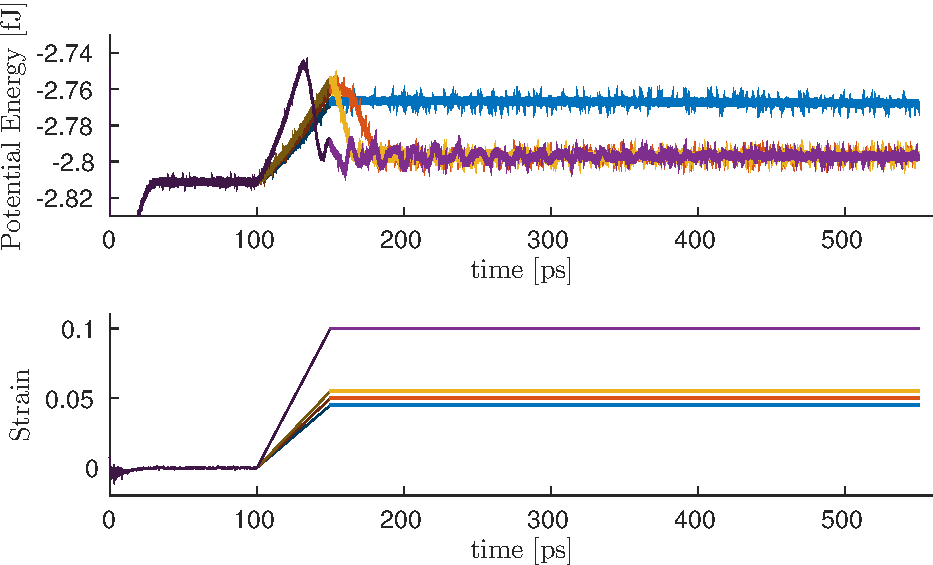
\includegraphics[width=\textwidth]{../figures/thesis/proof_of_concept_poteng_strain.pdf}
\caption{Potential energy (upper panel) and strain (lower panel) for a series of simulations where systems of 24x24x1 unit cells S1 hydrate are subjected to tensile strain. The systems were initiated with an elliptic crack of $6.0 \times 40.0 \si{\angstrom}$. The system was allowed to equilibrate NPT during \SI{100}{\pico\second}, which can be seen from the small fluctuations in strain in this timeframe. Then the simulations were NVT (but with imposed volume change due to straining). The thermostat and barostat damping times were \SI{1000}{\pico\second}. $T=\SI{260}{\kelvin}$. Falling potential energies correspond to crack opening (in these specific simulations). The systems that crack show oscillating potential energy after crack propagation, which is due to global oscillations of the system. The oscillations are damped out by a drag term in the thermostat.}
\label{fig:proof_of_concept_crack}
\end{figure}

\paragraph{Detailed crack analysis}
This is the point at which I developed my code to measure the crack area. Hopefully, that estimate will be better than the estimate solely based on the simulation box dimensions. The code also lets me follow the crack area in time, which makes it possible to measure the crack speed. I choose to define the crack speed as the change of crack area divided by the crack width, since the crack width is well defined – it is $L_z$ of the simulation box. Keeping in mind that my cracks travel in two directions, the crack velocity for a crack initiated as a hole parallell to the z-axis is:

\begin{equation}
v_c = \frac{1}{2L_z}\frac{\dd A_c}{\dd t}
\end{equation}

@MeasureCrackInTimeForTheseSimulations

\paragraph{Summary of concept simulations} The results from this initial simulation indicate that methane hydrate under these conditions are very brittle on the tens-of-picoseconds scale, in the sense that they do not at all plastcally deform to withstand strain. They either deform elastically, or they fail. There is also indications that the time before fracture depends on the applied strain in a systematic way. A close look at the potential energy curve of the simulation that did not end in rupture reveals that the potentail energy is actually slowly decreasing. Whether this is a sign of a coming fracture, strengthening rearrangements of particles -- which could imply some ductility -- or something else remains to be investigated.

